%!TEX root = /Users/dedan/bccn/lab_rotations/yifat/report/report_yifat.tex
\chapter{Methods} % (fold)
\label{sg:cha:methods}

% 
% ====================================
% = Description of the general setup =
% ====================================
\section{Animals, behavioral task and stimulation} % (fold)
\label{sg:sec:animals_and_behavioral_task}

The three monkeys (Maccaca fascicularis - subject id: C, D, V) used in the experiments performed an isometric wrist task with an instructed delay period where they held their hand in either a pronation or supination position and controlled a cursor on a computer screen. By applying a two-dimensional isometric torque at the wrist, they moved the cursor in the direction of one out of eight peripheral targets. A detailed description of the task can be found in a prior publication \citet{Yanai:2007p2455}.
% cortical chamber and mapping of the cortex
A cortical chamber was implanted above the motor cortex and the location of arm-related primary motor areas were mapped using a train of stimulating pulses (50 ms of biphasic stimulation given at 300 Hz with intensity $\leq$ 60 $\mu$A). This stimulation elicited an observable response (twitching of muscles) by which cortical areas could be related to forearm muscles. 
% EMG preprocessing
In both the behavioral task and stimulation condition, EMG activity was recorded simultaneously from forearm and hand muscles of the monkeys using sub-cutaneous intramuscular EMG electrodes (sixteen for C, twelve for D and eleven muscles for V). For naming of muscles see the table in theAppendix~\tref{app:tab:muscle_naming}. The EMG signals were then amplified, bandpass filtered, sampled at 10 kHz and stored. Details of the EMG recording technique have been described previously \citet{Prut:2003p2780}. It was checked whether synchronous activations in the EMG signal might be induced by electrical cross-talk. This was done by a blind source separation algorithm\citet{Chan:1995p3040} according to the method of Kilner et al.\citet{Kilner:2002p2941}. The possibly induced correlations were found to be insignificant and therefore further processing in order to remove crosstalk was omitted. All data-analysis was performed by self-written software using the MATLAB platform\citet{code}.
% figure of the setup 
\begin{figure}[p]
	\centering
		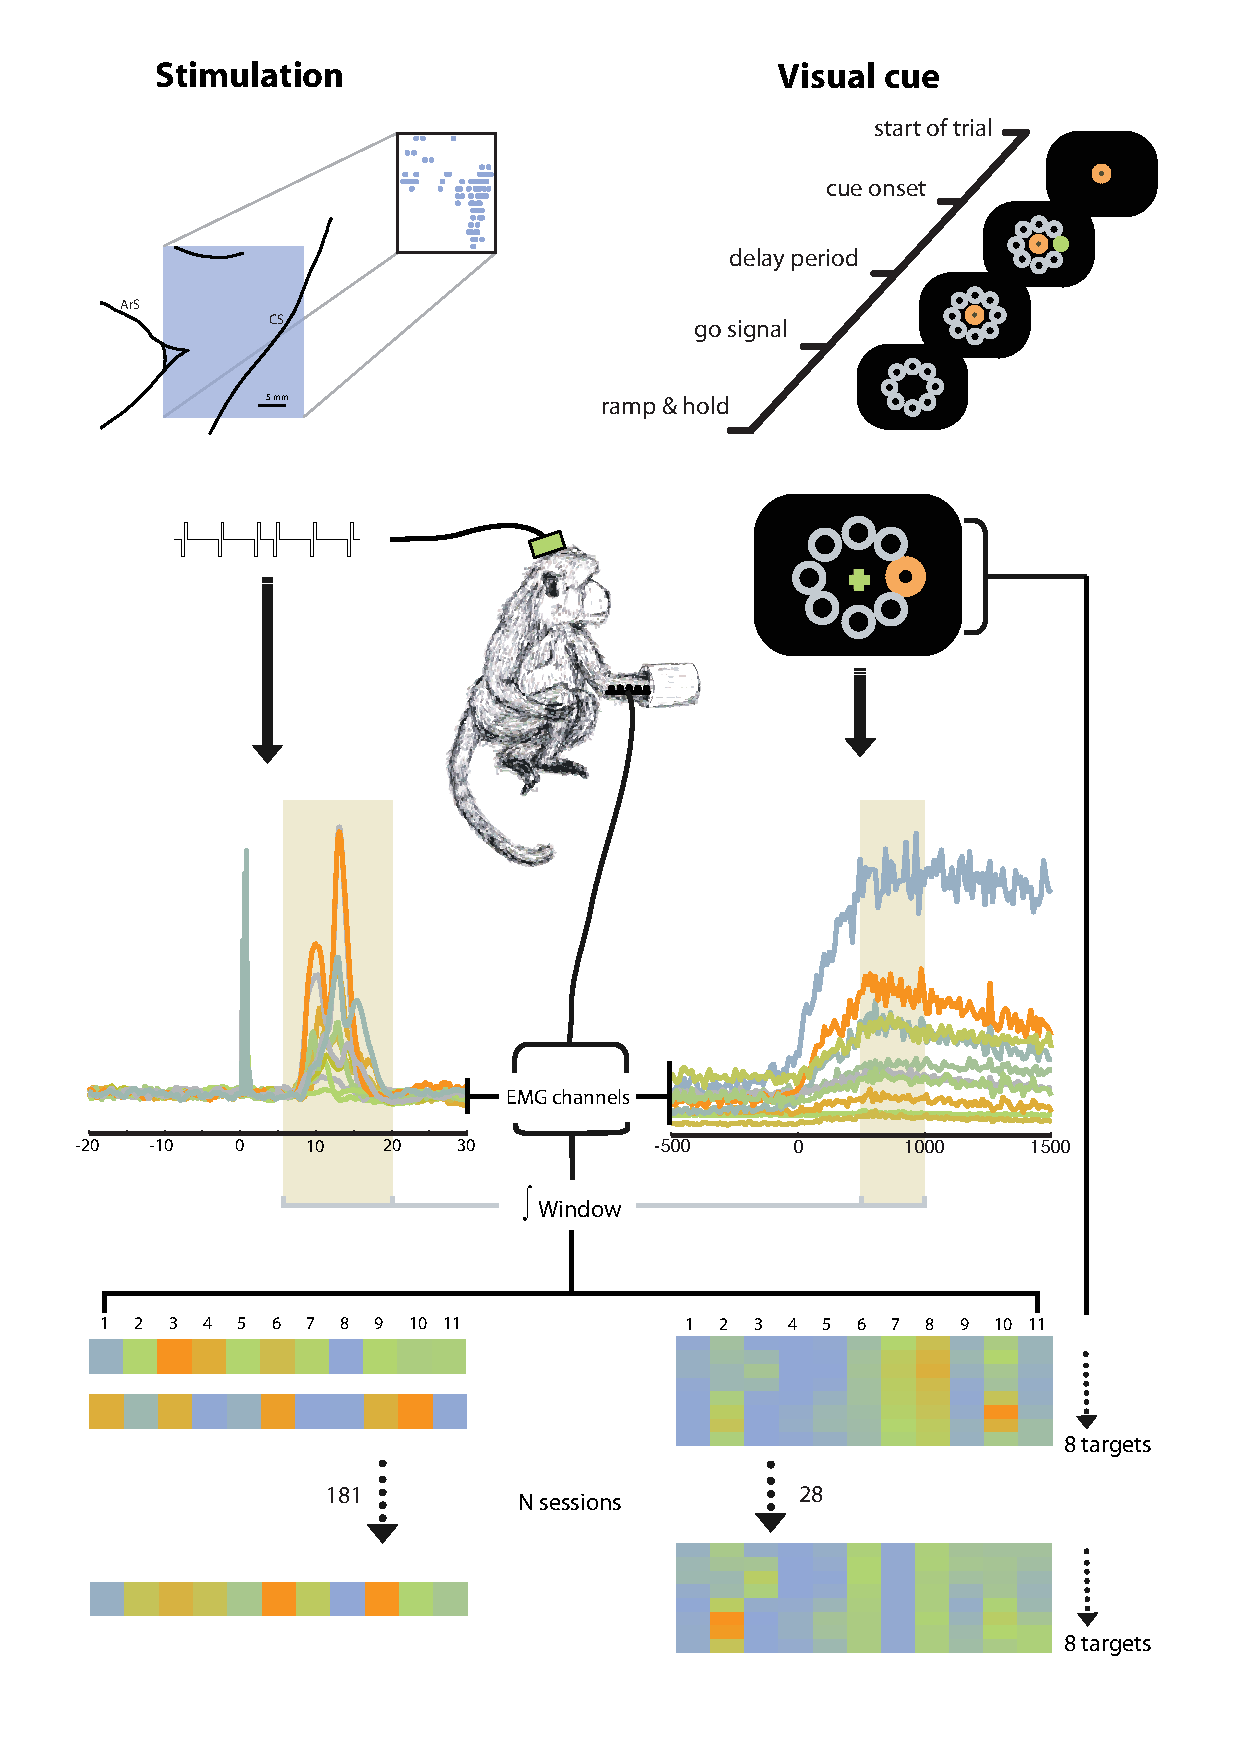
\includegraphics[width=0.9\textwidth]{images/setup.pdf}
	\caption{Experimental setup: Left side shows stimulation of arm related parts of the motor cortex while the monkey was performing the center-out task, which is depicted on the right side of the image. The gray bars show the window in which the signals were averaged for response pattern computation.}
	\label{sg:fig:images_setup}
\end{figure}

% section animals_and_behavioral_task (end)


%
%===============================================================================
% how did we record and what did we have to do with the data to make it useful =
%===============================================================================
\section{Recording and preprocessing} % (fold)
\label{sg:sec:rec_and_prep}

% 
% ========================================================
% = average window, response pattern in natural movement =
% ========================================================
\subsection{Muscle response pattern of natural movement} % (fold)
\label{sg:sub:natural_movement}


To compute a response pattern of muscle activations during natural movement, the torque onset (force on the joystick exerted by the monkey) was used as the trigger for average window computation. To get comparable results for different EMG channels, in spite of the fact that muscles have different background activation and variability they had to be normalized. A simple but reasonable and effective normalization technique is to define the response magnitude as change in mean activity in the post-trigger window compared to mean activity in the pre-trigger window. This method can deal with noisy channels without silencing them and is not affected by local DC offsets as only the change of activation is used as response magnitude. The mean activity in a 500 ms window after torque onset was divided by the mean activity in a time window of 500 ms before visual cue onset, as this showed to give the best baseline estimate. Every trial of the recording session resulted in one response pattern.

\subsubsection{Computation of preferred directions (PDs)} % (fold)
\label{sg:ssub:pds}

A preferred direction (PD) for each muscle was computed by a simple vector summation approach which yielded nearly similar results than a cosine fit used by Georgopoulos et al~\citet{Georgopoulos:1982p4165} in a similar study. For every muscle an average activity rate was computed for movement in each of the 8 directions~\rref{sg:fig:images_pd}. This activity rates can be seen as 8 points in a polar coordinate system with $r$ being the mean activity rate and $\theta$ corresponding to the target direction. These vectors were translated into the cartesian coordinate system where the vector sum was computed in order to give a measure of the \emph{weighted mean direction}. When translated back into the polar coordinate system, the obtained $\theta$ will give the preferred direction and the length of $r$ can be used to assess the significance of the tuning to a preferred direction. The $r$ value was compared to tuning significance of random muscle activation patterns in a bootstrapping test (5000 repetitions) and the PD significance of a session was set to the fraction of the bootstrapping results which had a higher $r$. 

\begin{figure}[ht]
	\centering
		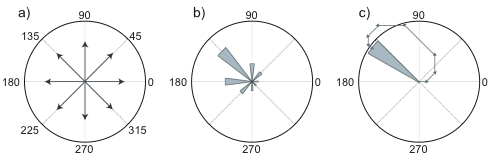
\includegraphics[width=0.8\textwidth]{images/pd.jpg}
	\caption
	{
	a) the 8 directions of movement. \\
	b) tuning curve of a muscle - mean activation in each of the directions. \\
	c) vector summation of tuning curve in cartesian space. \\
	}
	\label{sg:fig:images_pd}
\end{figure}
% subsubsection pds (end)

% subsection natural_movement (end)


% 
% ====================================================
% = stimulation, normalization, response fields, etc =
% ====================================================
\subsection{Muscle response patterns in the stimulation condition} % (fold)
\label{sg:sub:evoked_responses}

% the stimulation
During a subset of the recording sessions, sites of the motor-cortex which are related to arm and hand movement were stimulated by low frequency (0.3 Hz) trains of single biphasic pulses (each phase lasted 0.2 ms) at different amplitudes (50-250 $\mu A$). The single-pulse stimulation was used to excite local and small groups of cortical neurons. Using multi-pulse stimulations could recruit distant neurons as well so that the mapping would not be clear without ambiguity. Although it was found that also single-pulse stimulation and even small currents might activate groups of neurons~\citet{Tehovnik:1996p3982}, this method can still be used to investigate the response patterns of motor-cortical neurons because the motor cortex shows topographic organization into a patch-like structure where neighboring neurons share similar response properties~\citet{Lee:1998p4164}

% normalization
For each channel, the stimulation times served as triggers for the averaging of the zero-meaned and rectified EMG signals to compute the average response window and from this the muscle response pattern for a stimulation site. Each response pattern is a vector of real numbers where each number corresponds to the change in activity of a certain muscle in a post-stimulus window. After visual inspection of the average response around stimulation, the activity in a window between 6 and 20 ms after stimulation was chosen for the computation of response patterns, normalized by the 14 ms prior to stimulus onset. These latencies are consistent with other experiments\citet{Park:2004p3042}. The introduction of a 6 ms offset after stimulation avoids the filtering of an always present artifact induced by the stimulation. This thin spike, strictly time-locked to 0, does not affect the window after 6 ms. Some sessions, in which single channels contained wider artifacts or which seemed to be corrupted by noise, were sorted out by hand after visual inspection~\rref{sg:fig:images_artifacts}.
% stimulation artefacts and handsorting figure
\begin{figure}[ht]
	\centering
		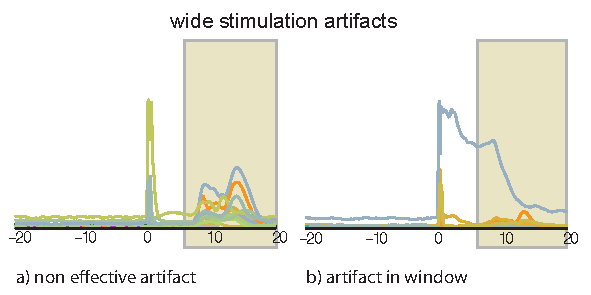
\includegraphics[width=0.7\textwidth]{images/artifacts.pdf}
	\caption{a) shows a typical thin spike artifact, strictly time-locked to 0, which does not affect the average window. \\
	b) depicts an artifact that would corrupt the computed muscle activation pattern and that was therefore sorted out
	after visual inspection}
	\label{sg:fig:images_artifacts}
\end{figure}


% remaining frequency components
Although the DC component of the EMG signal was removed previous to average response window computation by subtracting the mean of the channel activity, some channels occasionally showed a still remaining DC component in the  window \rref{sg:fig:images_dc_offset_fourier}. Analysis of raw data in the frequency domain showed that these channels with remaining DC offset contained large components in the frequency range between 10 and 500 Hz.
% fourier transform plot
\begin{figure}[ht]
	\centering
		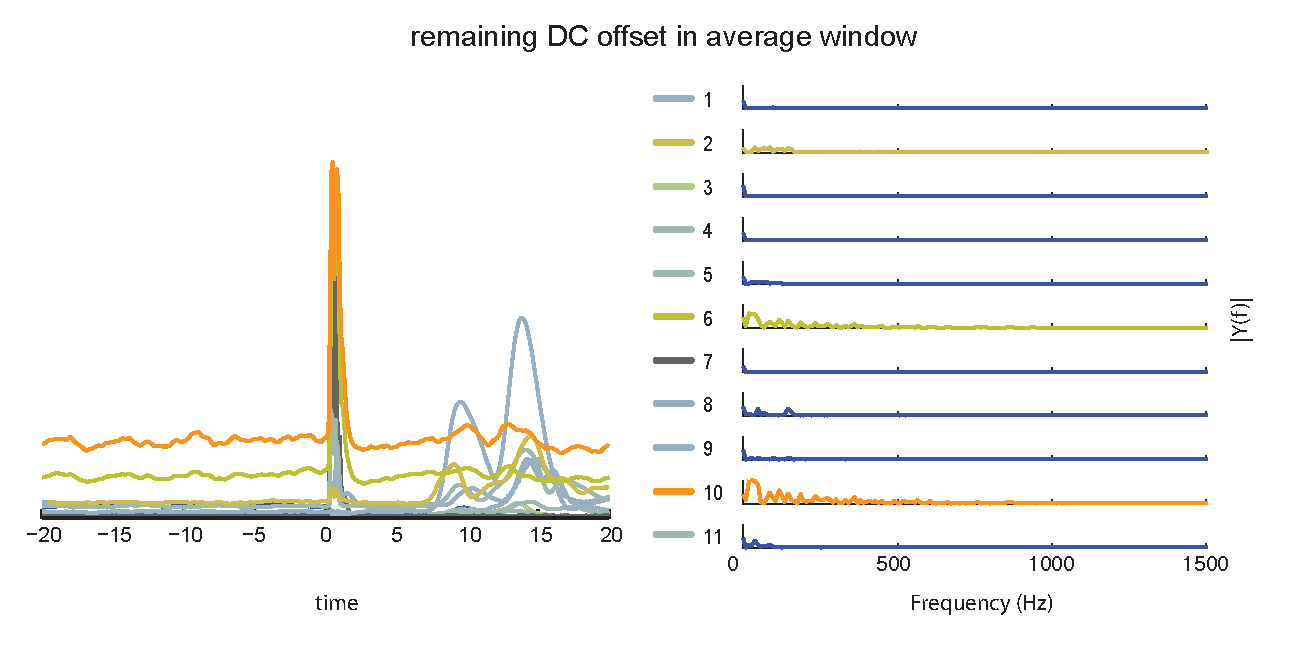
\includegraphics[width=0.9\textwidth]{images/dc_offset_fourier.pdf}
	\caption{Channels 10, 6 and 2 which show components in the frequency domain between 10 and 500 Hz have a remaining offset in the average response window.}
	\label{sg:fig:images_dc_offset_fourier}
\end{figure}
These superimposed frequency components cause the remaining DC offset as they are not removed by a simple subtraction of the overall mean. They could be removed by application of a low-pass filter to the raw data; however, this measure was omitted as it did not influence the computation of muscle response patterns by the selected normalization technique.



% =======================
% = the response fields =
% =======================
\subsubsection{Response fields} % (fold)
\label{sg:subs:response_fields}

Response fields are defined as the size of the response elicited by cortical stimulation. The size was measured as the number of channels that showed a significant reaction to the stimulation. To identify the stimulus induced response for each channel separately, the average activity in a time window (-20 to -6 ms) prior to stimulus onset was compared with the average activity in a time window (6 to 20 ms) following stimulus onset. The comparison of these activations was performed across stimulus repetitions using a two-sided rank sum test (Wilcoxon rank sum test implementation of MATLAB 2008b). The muscle field size for a session was determined as the number of channels with significant responses (p < 0.05). Recordings from stimulation sites with a response field of size 0 have been discarded.

% subsubsection response_fields (end)

% subsection evoked_responses (end)

% section rec_and_prep (end)


% 1
% =================================================================
% = how the synergies were computed and compared among each other =
% =================================================================
\section{Identification of muscle synergies} % (fold)
\label{sg:sec:factorization}

% 1
% ===================================================
% = about the general idea of matrix factorizations =
% ===================================================
\subsection{matrix factorizations in general} % (fold)
\label{sg:sub:mf}

As in previous studies mentioned above, whose goal was to search for muscle synergies, matrix factorization (MF) techniques were used to search for the possible underlying structure present in the data. This class of algorithms assumes that the data is a result of linear combinations of a few patterns which are distorted by noise. This can be modeled by the following equation,
\begin{equation}
	\vec{x} = \sum_{i=1}^n c_{i} \vec{w}_{i} + \vec{\varepsilon}
\end{equation}
where $\vec{x}$ is a N-dimensional data vector composed of the i-th basis vector $\vec{w}_{i}$, its scalar activation coefficient $c_{i}$ 
and $\vec{\varepsilon}$ is an unknown noise component vector.


Algorithms that assume a linear summation of muscle synergies attempt to recover the identity of the synergies using matrix factorization techniques that aim to explain the variability in muscle activity in different task conditions by variable activation of a smaller number of muscle synergies. The algorithms differ in the assumptions they make about the distribution of noise and activation coefficients of the data and consequentially yield different features. Two factorization algorithms were used in the study, whose constraints appeared to be biologically plausible and that were previously tested on synthetic and experimental data~\citet{Tresch:2006p3766}. They showed good performance on data sets having the special properties of muscle activations patterns (e.g. non-negativity, signal-dependent noise and possibly correlated activation coefficients) and were suggested to yield better results than other methods. Although the algorithms with best performance led to stable and reliable results, the two chosen factorizations where always applied in parallel to make sure that the result is not an artifact of the used MF-algorithm. 

The general form of the matrix factorization is: $A = W H$ where 

\begin{description}
	\item[A] is the activity matrix showing the change of mean EMG activity of each muscle (rows) for each task condition or stimulation site (columns). 
	\item[W] is a matrix with columns forming a base of muscle synergies. Each column is a single muscle synergy that shows the constant relations between different muscle activations when this specific synergy is activated.
	\item[H] is a loading matrix whose entries show the level of activation of a given synergy (row) in a given task condition or stimulation site (column). 	
\end{description}
  
Since the number of synergies are expected to be smaller than the number of muscles, the multiplication of matrices $W$ and $H$ only forms an approximation of $A$.
\begin{equation}
	A \approx W H \text{ with } A: m \times n, W: m \times l \text{ and } H: l \times n \text{  } | \text{  } l \leq m
\end{equation}
The reconstruction error between matrix $A$ and its approximation (called the model from here) $W H$ decreases as the number of synergies (l) increases. This \emph{remaining-error} was used to assess the quality of the model and was defined as $1 - \text{explained variance}$. The \emph{remaining-error} of a model was always compared to random data exposing the same statistical properties, created by shuffling within the channels, to make sure that the results were not induced by statistical properties of the recorded data. This shuffling was repeated 100 times in order to get a better estimate of how much the remaining-error values were influenced by statistical characteristics instead of underlying structure. 

% subsection mf (end)

% 1
% ========================================
% = the nmf algorithm and its properties =
% ========================================
\subsection{Non negative matrix factorization (NMF)} % (fold)
\label{sg:sub:nmf}

The main advantage of NMF is the strong assumption of non-negativity \citet{Lee:1999p1635}, on both basis vectors and activation coefficients, which fits the muscle activation patterns. This assumption can be biologically interpreted as a constraint on the muscles such that each muscle may only be recruited to pull but not to push. Since components only add positive values, they cannot be combined to cancel each other. This property causes components to represent local features in the input space.

To solve the factorization problem the built-in NMF implementation of MATLAB 2008b (nnmf - Statistics Toolbox) was used. The NMF-algorithm tries to minimize the error function given by the square Euclidian distance between matrix $A$ and its approximation $WH$ and has been proven to converge to local minima of this function~\citet{Lee:2001p1638}. In order to search for a global minimum an exploration period was introduced. During this exploration phase 100 runs of the algorithm were repeated with different initializations. Within every run only 50 iterations were executed by using a more unstable multiplicative update rule, in order to enforce exploration. The best result of the exploration was then used as the initialization for 100 additional iterations, which used the more stable and faster converging alternating update rule. The stability of this method was shown by repeating the whole procedure 20 times ultimately leading to 20 times l vectors with l being the number of assumed synergies (model order). This way the approximation of a $11 \times 100$ matrix to a linear combination of 3 (l) distinct 11 dimensional vectors led to $3 \cdot 20 = 60$ candidates for synergy vectors. These candidates can be interpreted as data-points in a 11 dimensional space. Afterwards the unsupervised learning method of vector quantization (k-means, MATLAB 2008b implementation) was applied to these data-points, in order to see whether 3 groups or clusters can be found which would correspond to 3 constantly detected synergies~\rref{sg:fig:images_nmf_expl_stab3}. In case of l stable groups a k-means clustering with l prototypes would therefore lead to a constant number of data-points assigned to each prototype and therefore the standard-deviation of data-points per cluster was chosen as a stability measurement for the NMF-algorithm. In all cases where NMF was applied in this study the standard-deviation has been found to be 0, indicating a very stable result of the chosen exploration method. The prototypes of the clustering, representing the average of a cluster, were used as synergies for following analysis.
% k means exploration stability figure
\begin{figure}[ht]
	\centering
		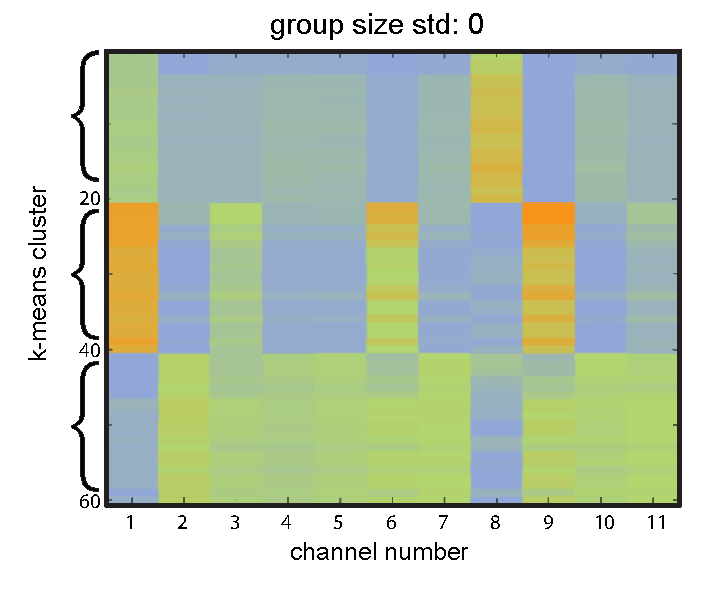
\includegraphics[height=3in]{images/nmf_expl_stab3.pdf}
	\caption{The stability of the used nmf exploration procedure was proofed by running the algorithm for 20 times repeatedly and afterwards grouping the resulting synergy vectors according to prototypes of a k-means clustering. The standard deviation of the group size was used as a stability measure and was 0 in all cases where NMF was applied within this study.}
	\label{sg:fig:images_nmf_expl_stab3}
\end{figure}

% subsection nmf (end)

% 1
% ========================================
% = the pcaica method and its properties =
% ========================================
\subsection{Independent component analysis in the subspace of principal components (PCAICA)} % (fold)
\label{sg:sub:pcaica}

Although muscles in general do not posses \emph{negative activation}, during some movements they might be less active than their average activity during movement. In contrast to NMF, the PCAICA algorithm is also capable of detecting and showing these inhibitory effects in muscle activation patterns. 

First the dimensionality of the data was reduced by principal component analysis (PCA), which can be described as a dimensionality reduction with the objective to lose as little information as possible. Therefore the data is transferred into a lower dimensional subspace whose orthogonal basis is oriented in the direction of the largest variance by minimizing the correlation of the data-points (muscle activation patterns). This basis is chosen in such a way that the first basis vector explains the largest possible part of the variance of the data, the second one explains the possible largest part of remaining variance, and so forth. Afterwards the independent component analysis (ICA) was applied to this subspace in order to increase the statistical independence of the PCA coefficients (also know as loadings). Principle component analysis was applied to the data matrix $A$ by using the MATLAB function \emph{princomp} for which the number of variables corresponds to the number of muscles and the number of observations to the number of trials. This function also applies the required conversion to a zero-meaned distribution as it is required for PCA so it can directly be used with the same data as the NMF-algorithm. Subsequently the \emph{runica} function from the eeglab package~\citet{eeg} in its extended version was used on the scores of the first N selected eigenvectors. 
\todo{better explanation why and how we used ica}
This procedure generates components that may have negative values. However, since both PCA and ICA operate on signals with zero mean, a negative value for a given muscle can be interpreted as being activated less that its overall positive non-zero mean and can therefore reflect a inhibition of the muscle. The ICA section of the algorithm does not alter the reconstruction error that is determined by the eigenvalues of the first N selected principal components.
% subsection pcaica (end)

% 1
% ===============================================================
% = how to decide to which dimension we want to reduce the data =
% ===============================================================
\subsection{Model order selection/detection} % (fold)
\label{sg:sub:model_order}

Another reason to apply several algorithms in parallel is the difficulty to chose the correct dimensionality to which the data should be reduced, which is also known as the problem of model-order selection. As there is still no optimal solution for this decision Tresch et al proposed to compare results of different techniques. To asses the number of synergies the plot of reconstruction errors was used. In this plot of reconstruction error vs. number of used synergies the error decreases as more synergies are added. A marked slope change in this curve may point to the correct number of synergies, since adding more synergies does not significantly improve the reconstruction. Tresch et al developed an ad-hoc method for automatic detection of the change in slope, which gave good results in their work, where the decisive slope change could be estimated from the known true number of synergies. As a reliable parameter could not be found for the data of this work, the ad-hoc method was not used. Though an objective measure for model order selection could not be used, the chosen order seamed reasonable as a minimal number of synergies was selected by a clearly visible \emph{elbow} in the remaining error plot. Furthermore the previously mentioned paper of Tresch et al also showed that equal or similar synergies may also be found despite a wrong choice for the model order. Experiments took place within my study where data was reduced to both a higher number of synergies and also to a lower order model. The best synergies (with respect to most explained variance (NMF) or highest eigenvalues (PCA)) from the higher order model were compared to the synergies of the lower order model. These experiments came to the same results as in the publication of Tresch et al.

% subsection model_order (end)


% 1
%===============================================================================
% = comparison of synergies, detected by different methods or in different posture =
%===============================================================================
\subsection{Synergy comparison} % (fold)
\label{sg:sub:comp}
To compare two groups of synergies obtained by different methods, the vectors were first normalized ( $\abss{x} = 1$ ) and then compared by using the dot product between them as a similarity measure. Comparison of two sets of synergies that were obtained by different algorithms, was realized by matching each vector of the first set against the vector most similar to it from the second set, in decreasing similarity order starting with the pair having maximal similarity. However the dot product was only used as a similarity measure for the grouping. As a matching score, shown also in the plots, the correlation coefficient was used as it showed to be less influenced by statistical properties of the synergies. This method showed good results in terms of grouping similar synergies together, that could also be detected as very similar by visual inspection, although it does not give an objective and quantitative measure as the similarity measure is biased by the statistical properties (mostly non-negativity) of the synergy vectors. For quantitative analysis it is planned to make use of bootstrap methods as used in other studies~\citet{AdAvella:2005p2330}. Furthermore the correlation between two groups was computed on two vectors that contained all connected muscle activation patterns of a group.
\todo{when I apply my bootstrap method, explain here how it was done}
% explanation of matching score figure
\begin{figure}[ht]
	\centering
		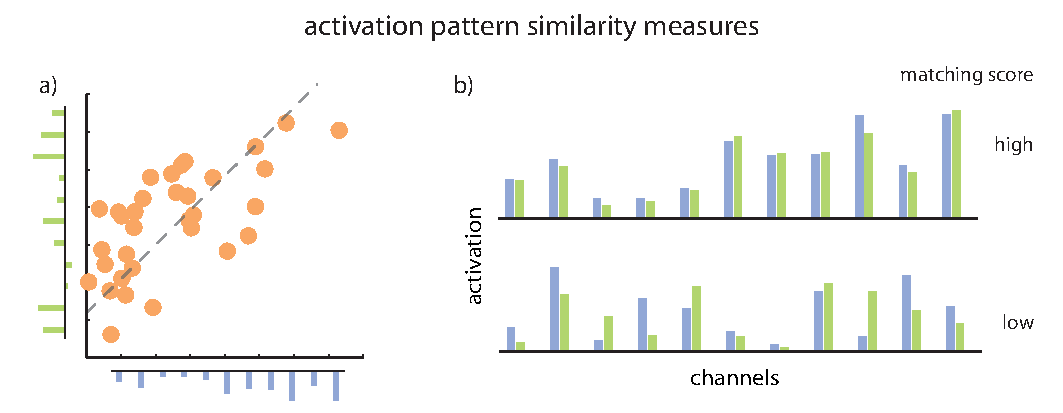
\includegraphics[width=0.8\textwidth]{images/match_explanation.pdf}
	\caption{This plot shows how similarity of muscle activation patterns or synergies is measured. a) by correlation of a group of activation patterns, connected together in one vector. b) correlation coefficient of single activation patterns, grouped by best fitting similarity in the two sets. }
	\label{sg:fig:images_match_explanation}
\end{figure}

% subsection comp (end)



% section factorization (end)



% ===============================================================
% = comparison of synergies in different space (pd, projection) =
% ===============================================================
\section{Analysis of synergies in interesting spaces} % (fold)
\label{sg:sec:syn_comp}


% ========================================
% = cstd, roseplots, prefered directions =
% ========================================
\subsection{Muscle synergies in the space of preferred directions (PDs)} % (fold)
\label{sg:sub:pd}

As a measurement of \emph{directedness} of a certain muscle activation pattern, the circular standard deviation (\emph{cstd}) of PDs belonging to muscles activated within this pattern was computed. All circular statistics were done by using~\citet{circ_stat}. The \emph{cstd} for a given vector $\vec{x}$ of radians is defined by 
\begin{equation}
	\emph{cstd} := \sqrt{-2 \ln{\bar{R}}}
\end{equation}
where the mean resultant length $\bar{R}$ is given by 
\begin{equation}
	\bar{R} := \frac
					{ \sqrt{ {(\sum_{i}^n \cos  \vec{x}_i)}^2 + {(\sum_{i}^n \sin \vec{x}_i)}^2 }}
					{n}
\end{equation}
The \emph{cstd} was computed only on muscles of a synergy having an activation coefficient greater than the median of all muscle activation coefficients. This \emph{cstd} of a synergy was then compared
to a distribution of \emph{cstd}s from random samples of muscles drawn from a distribution with similar statistical properties to the synergies.


\begin{figure}[ht]
	\centering
		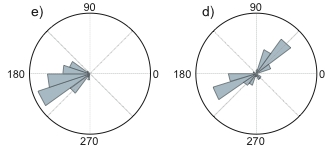
\includegraphics[width=0.8\textwidth]{images/cstd.jpg}
	\caption
	{
	d) a muscle activation pattern with small circular standard deviation \\
	e) a muscle activation pattern with large \emph{cstd}.
	}
	\label{sg:fig:images_cstd}
\end{figure}
% subsection pd (end)


% 1
% ===========================================================
% = synergy similarity, orthogonal projection and bootstrap =
% ===========================================================
\subsection{Projection of evoked responses on natural synergies} % (fold)
\label{sg:sub:projection}

The question, whether the cortical stimulation induced responses are just arbitrary activations of muscles that contain some structure but are not related to natural activation patterns or whether they have something in common with the activation patterns that were found during natural movement is an interesting question. If this were the case, it would imply that the stimulation sites are in fact the sites where neuronal activation causes modular organized muscle response patterns, if these happen to be found during natural movement. The idea is to project the evoked responses to the subspace which is spanned by the natural synergies. When this transformation does not change the data, it already resides within this subspace. In more technical language, the data was orthogonally projected to an orthonormal basis constructed from the natural synergies and also to the orthogonal complement of this basis. How much the data tends to reside within one of the two subspaces is measured by the ratio between the sum of vector lengths (L2 norm) over all responses after projection to the two bases.

\begin{equation}
	ratio = \frac
		{\sum_{i} \abss{P(\vec{x}_{(i)})}} 
		{\sum_{i} \abss{P^{\perp}(\vec{x}_{(i)})}}
\end{equation}

As the chance to already reside within a m-dimensional subspace of an n-dimensional space highly depends on the ratio between $m$ and $n - m$ it was first tried to compare the ratio of the data to an expected ratio. If the entries in the natural movement synergy vectors would be drawn from a normal distribution with zero mean, the expected ratio would be exactly the ratio $\frac{m}{n - m}$. But when using the non-negative synergy vectors from natural movement this ratio becomes shifted. This is due to the Gram-Schmidt process which is used for the orthonormalization of the synergies. It always creates the first basis vector in the positive (hyper-)quadrant, which leads to an offset. As the main interest of the method was a qualitative answer, it was not further pursued to find an estimate for the offset from our data, but a bootstrap method was applied to find whether the data resides in the subspace of interest on a level above chance. Therefore the ratio computed for the data was compared to distributions of ratios, coming from 10000 runs of the projection on random data with the same statistical properties. As random data was used:

\begin{itemize}
	\item random data with same mean and std as original data
	\item random data with same mean and std within channels as in the original data
	\item shuffled versions of the original data
	\item within channel shuffled versions of the original data
\end{itemize}


% subsection projection (end)





% section syn_comp (end)



% section methods (end)
